\documentclass[a4paper,english,12pt]{report}
%

\usepackage{amsmath}
\usepackage{amsfonts}
\usepackage{epsfig}
\usepackage{multicol}
\usepackage{wrapfig}
\usepackage{enumerate}
\usepackage{enumitem}
\usepackage[utf8]{inputenc}

\usepackage{geometry}

\geometry{
a4paper,
total={210mm,297mm},
left=20mm,
right=20mm,
top=20mm,
bottom=20mm,
bindingoffset=0mm
}

\newcommand{\meshup}[0]{\textsc{MeshUp}}
\newcommand{\cmake}[0]{\textsc{CMake}}
\newcommand{\rbdl}[0]{\textsc{RBDL}}
\newcommand{\muscod}[0]{\textsc{MUSCOD-II}}

%\def \Tfree {T^{\textup{free}}}
\def \Tfree {t^f}
\def \st {\textit{subject to:}}

\begin{document}
\thispagestyle{empty}

%%%%%%%%%%%%%%%%%%%%%%%%%%%%%%%%%%%%%%%%%%%%%%%%%%%%%%%%%%%%%%%%%%%%%%%%%

\section*{\rbdl{} and \muscod{}: Example 2: Cart Pendulum} 



Debora Clever, Manuel Kudruss  (debora.clever@iwr.uni-heidelberg.de)

\begin{wrapfigure}{r}{0.3\textwidth}
	\begin{center}
		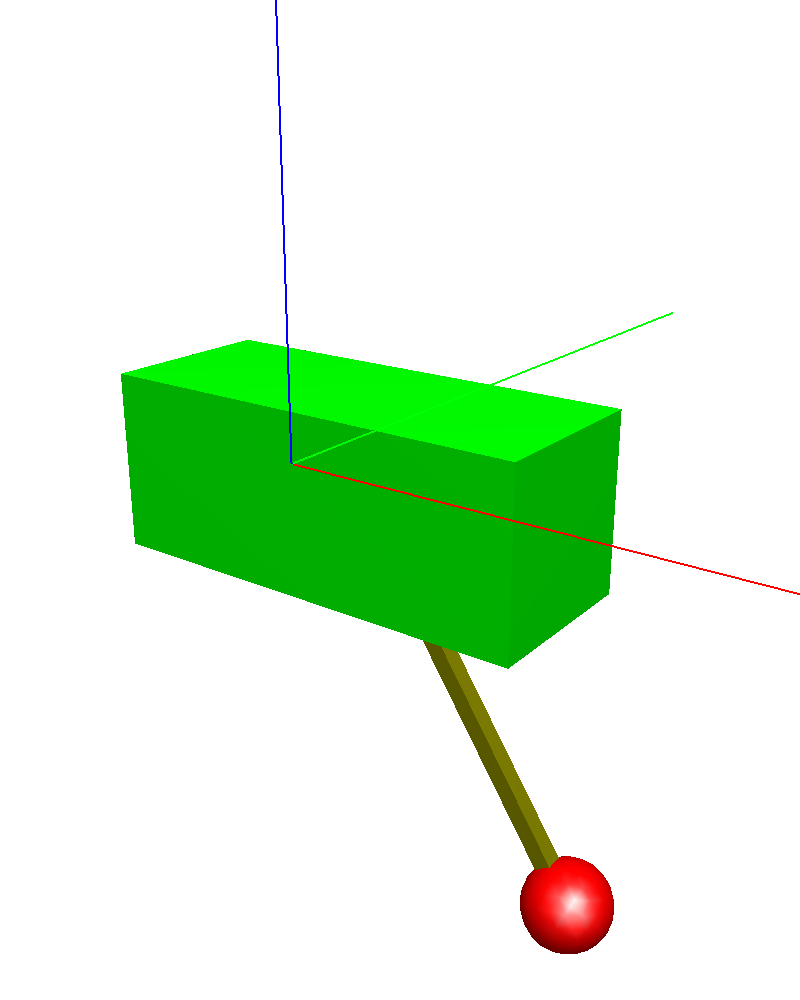
\includegraphics[width=0.2\textwidth]{cart_pendulum_base}
	\end{center}
	\caption{Cart Pendulum}
	\label{fig:cartpendulum}
\end{wrapfigure}

\bigskip
\bigskip

This is a simple example that should get you started with MUSCOD and RBDL. It is devoted to the introduction to forward dynamics and one-phase optimal control problems. To this end we consider a cart pendulum, see Figure \ref{fig:cartpendulum}.

The cart pendulum consists of two rigid bodies, the \emph{Cart} and the
\emph{Pendulum}. The pendulum itself consists of two elements, a spherical mass and a massless link. The model has two degrees of freedom:
\begin{itemize}
 \item $q_0$: the $x$-translation of the body \emph{Cart}.
 \item $q_1$: the rotation around the $y$ axis of the body \emph{Pendulum}.
\end{itemize}

\bigskip

The movement of the pendulum can be controlled by a force $u_0$ acting in horizontal direction on the cart. 

\bigskip

\emph{Cart:} 
\begin{itemize}
 \item Cuboid
 \item $x$-length= 0.5m, $y$-length = 0.2m, height = 0.2m
 \item mass = 10.0kg
\end{itemize}

\emph{Pendulum:}
\begin{itemize}
 \item Massless link: length = 0.5m
 \item Sphere: radius = 0.1m, mass = 1.0kg
\end{itemize}


\subsection*{Tasks}

At initial time $t_0=0$ the pendulum is hanging down. Determine an optimal control, such that at final time $t_f$, the pendulum is standing up. To this end:

\begin{enumerate}
	\item Set up a feasible lua model, describing the cart pendulum model.
	\item Complete source and data file.
	\item Optimization 1: Minimize energy consumption.
	\item Optimization 2: Minimize final time.
\end{enumerate}
\medskip

\end{document}
